\subsection{Softwarearchitektur}

Seitdem die ersten Großrechner gebaut wurden und ein Projekt nicht mehr von einem Team allein entwickelt werden konnte, entstand der Bedarf komplexe Systeme aufzuteilen und zu strukturieren. So war es schon in den 60er Jahren notwendig, die Entwicklung des Betriebssystems OS/360 von IBM auf mehrere Teams aufzuteilen und klare Schnittstellen zwischen den Teilen zu bestimmen \parencite{brooks_mythical_1995}. Es entwickelte sich daraus eine der ersten Anwendungen und Umsetzungen von Softwarearchitektur, welche erstmalig 1969 bei einer Softwaretechnik Konferenz in Rom auch als solche bezeichnet wurde \parencite[vgl.][S. 12]{buxton_software_1970}.

In den darauffolgenden Jahren wuchs das Interesse an der Thematik und die Anwendungen der Teilung und Strukturierung von Software-Systemen. Hieraus entstand die im Jahr 2000 veröffentlichte Norm IEEE1471:2000, welche am 15. Juli 2007 als ISO/IEC 42010 übertragen wurde. In diesem Standard werden Anforderungen an die Beschreibung von System-, Software- und Unternehmensarchitekturen definiert \parencite{hilliard_isoiecieee_nodate}.

\subsubsection{Definition}
\label{sec:software-architect-definition}

Nach der Norm IEEE1471:2000 handelt es sich bei dem Begriff Softwarearchitektur, um eine  \textit{\enquote{grundlegende Organisation eines Systems, die in einzelne Komponenten und ihren Beziehungen untereinander unterteilt ist}}, sowie der technischen Umsetzung und weiterführenden Prinzipien hinsichtlich des Programmierparadigma \parencite[][S. 12]{clements_comparing_2005}.

Helmut Balzert, einer der führenden Pioniere im Bereich Softwarearchitektur und Autor der Bücherreihe \textit{Lehrbuch der Softwaretechnik}, beschreibt diese als \textit{\enquote{eine strukturierte oder hierarchische Anordnung der Systemkomponenten, sowie Beschreibung ihrer Beziehungen}} \parencite[][S. 580]{balzert_lehrbuch_2011}. Nach Balzert lässt sich somit jedes System in mehrere einzelnen Komponenten teilen, welche untereinander in Verbindung stehen und gemeinsam das Gesamtsystem formen.

Paul Clements, Autor der IEEE Norm, schließt sich Balzert an und beschreibt Softwarearchitektur als \textit{\enquote{Strukturen eines Software-Systems: Softwareteile, die Beziehungen zwischen diesen und die Eigenschaften der Softwareteile und ihrer Beziehungen}} \parencite[][S. 23]{clements_documenting_2010}.

Neben diesen rein technischen Betrachtungen des Begriffes, gibt es eine von Martin Fowler, die mehr den soziale Austausch beim Entwicklen hervorhebt und Softwarearchitektur als  \textit{\enquote{geteiltes Verständnis von hart zu änderten Entscheidungen}} sieht \parencite[][S. 3]{fowler_who_2003}. Dabei gibt Fowler keinerlei Vorgaben hinsichtlich jeglicher Untergliederung, sondern beschreibt mehr den Austausch, durch welchen Softwarearchitektur im Unternehmen ausgeführt wird. Nach Fowler handelt es sich dabei um einen offenen Disput, indem jede Entwicklerin oder jeder Entwickler die Rolle des Softwarearchitekten einnehmen kann \parencite[][S. 3 f.]{fowler_who_2003}.

Somit wird, abgesehen von der Betrachtung von Fowler, Softwarearchitektur als Strukturierung von einzelnen Komponenten, die untereinander in Beziehung stehen, definiert. Dabei können sowohl die Komponenten, als auch die Beziehungen Eigenschaften besitzen. Die einzelnen Komponenten zusammen ergeben das Gesamtsystem, welches in einer bestimmten Struktur vorliegt und beschrieben wird. Folglich beinhaltet die Softwarearchitektur alle nötigen Informationen über die Struktur der einzelnen Systemkomponenten und deren Kommunikationen untereinander.

Wird ein Software-System in Komponenten geteilt, welches jedoch selbst eine Funktionalität besitzt, bedeutet dies, dass auch diese Logik in Teile geteilt wird und jede einzelne Komponente einen Teil erfüllt. Um gleichermaßen den selben Funktionsumfang, wie das Gesamtsystem bewältigen zu können, müssen die einzelnen Komponenten zusammenarbeiten. Es ist deshalb wichtig, die Zuständigkeit jeder einzelnen Komponente genau zu klären und die Abhängigkeiten zu bestimmen. Auf Grund der Abhängigkeiten werden im Anschluss Schnittstellen definiert, über die die einzelnen Komponenten Informationen austauschen können.

Bei der Teilung in einzelne Komponenten können bekannte Architekturstile helfen, da sich diese im Laufe der Zeit entwickelt haben und gut dokumentiert sind. Architekturstile sind Regeln zur Strukturierung eines Systems. Sie fassen Merkmale eines IT-Systems sowohl hinsichtlich der Komponenten, als auch ihrer Kommunikation zusammen \parencite[vgl.][S. 102]{starke_effektive_2015}. Seit Beginn der Softwarearchitektur hat sich eine Vielzahl an solchen Stilen entwickelt, die aus unterschiedlichen Intentionen entstanden sind. Jedes System hat dabei unterschiedliche Herangehensweisen, sowie Vor- und Nachteile. 
Auch können verschiedene Architekturstile zum lösen des gleichen Problems genutzt werden. Hinsichtlich der Auswahl des Stiles gibt es keine richtige oder falsche Antwort. Es ist viel mehr das Abwägen von Vor- und Nachteilen und der Präferenz der Entwickler.

Da die unterschiedlichen Architekturstile nicht im  Fokus dieser Bachelorarbeit sind, werden nur folgende Stile betrachtet:

\begin{enumerate}
	\item Verteilte Systeme,
	\item Interaktionsorientierte Systeme,
	\item REST-Architektur,
	\item Monolithische Architektur
\end{enumerate}


\subsubsection{Verteilte Systeme}
\label{sec:verteilte-systeme}

Nach Andrew Tanenbaum werden verteilte Systeme als eine Menge unabhängiger Computer bezeichnet, die dem Benutzer wie ein einzelnes, kohärentes System erscheinen \parencite{tanenbaum_verteilte_2007}.

Weiterführend beschreibt Gernot Starke die einzelnen Komponenten als entweder Verarbeitungs-, oder Speicherbausteine, die über definierte Schnittstellen innerhalb eines Kommunikationsnetzes zusammenarbeiten \parencite[vgl.][S. 116]{starke_effektive_2015}.

Im Gegensatz zur Definition von Softwarearchitektur grenzt sich das verteilte System dadurch ab, dass von unabhängigen Computern geredet wird. Dadurch entstehen einige Vorteile. So lassen sich auf Grund der Unabhängigkeit, diese einzelnen Rechner unterschiedlich skalieren. Es entsteht ein Netzwerk an heterogenen Computern. Somit kann je nach Anforderung der einzelnen Komponenten, eine entsprechende Rechenleistung genutzt werden.

Des Weiteren gibt es auf Grund der Verteilung eine gewisse Ausfallsicherheit. Diese entsteht, weil das Gesamtsystem nicht durch eine, sondern durch mehrere Maschinen getragen wird. Es können einzelne Computer ausfallen, ohne dass das Anwendungssystem ausfällt. Dies hängt natürlich von der ausgefallenen Funktionalität ab. So kann bei Ausfall eines kritischen Teils,  im schlechtesten Fall das gesamte Anwendungssystems funktionsunfähig sein. Um dies zu verhindern, sollten geeignete Maßnahmen getroffen werden und kritische Funktionen auf mehreren Computern implementiert sein.

Jedoch entsteht mit der Verteilung auch ein Anstieg der Komplexität sowohl bei dem Konzipieren des Systems, als auch bei der Wartung und Verwaltung dessen. Außerdem muss nicht nur ein Rechner abgesichert werden, sondern ein ganzes Netzwerk. Dadurch entsteht ein höherer Aufwand zur Absicherung.

Die einzelnen Computer können über verschiedene Mechanismen miteinander kommunizieren: Einerseits durch direkten Aufruf entfernter Funktionalität und andererseits durch indirekten Austausch von Informationen \parencite[vgl.][S. 116]{starke_effektive_2015}. Dabei kann der Transfer synchron oder asynchron ablaufen. Bei einem synchronen Aufruf, der nur direkt ausgelöst wird, führt ein Computer über das Netzwerk die Funktionalität eines anderen aus und wartet auf dessen Antwort \parencite{synchrone_2018}.
Bei einem asynchronen Aufruf wird entweder direkt oder indirekt Logik eines anderen Computer aufgerufen, während der aufrufende Rechner, ohne auf die Antwort zu warten, weiter verarbeitet. Ist der aufgerufene Rechner fertig, gibt er das Resultat zurück, welches vom ersten Computer aufgenommen und verarbeitet wird \parencite{wiki_asynchrone_2019}.

Der Austausch von Informationen und das Aufrufen von externer Funktionalität kommt in einem System dauerhaft vor. Dadurch besteht das Risiko, dass einzelne Nachrichten zwischen den Komponenten verloren gehen und das System sicherstellen muss, dass dieser Datenverlust abgefangen wird.

\subsubsection{Interaktionsorientierte Systeme}
\label{sec:mvc}

Interaktionsorientierte Systeme zeichnen sich dadurch aus, dass sie den Fokus auf die Interaktion zwischen Mensch und Maschine legen \parencite[vgl.][S. 124]{starke_effektive_2015}.
Ein viel verwendeter Vertreter hiervon ist der Model-View-Controller-Ansatz (MVC-Ansatz). Hierbei werden die einzelnen Komponenten in drei unterschiedliche Kategorien eingeteilt, von dem jeweils ein Repräsentant vorhanden sein muss. Eingeteilt wird in die drei Kategorien: Model, View und Controller, wobei jede Gattung eine eigene Funktionalität besitzt.

So kümmert sich das Model um die Datenspeicherung, den Datenabruf und die Verarbeitung von Informationen und ist eine Verbindung zwischen dem Speichermedium und der Anwendung (siehe \cref{fig:mvc-cm-kommunikation} und \cref{fig:mvc-vm-kommunikation} Punkt 4 und 5 bzw. Punkt 5 und 6). Da jegliche Speicherung ausschließlich über das Model abläuft, wird das Speichern und das Abrufen einheitlich geregelt.

Davon getrennt sind die graphischen Darstellungen, welche durch Views definiert werden. Sie erhalten die Informationen vom Model. Dabei können die Daten entweder direkt von der View angefordert (siehe \cref{fig:mvc-vm-kommunikation} Punkt 4) oder indirekt vom Controller übergeben werden (siehe \cref{fig:mvc-cm-kommunikation} Punkt 3 und 7). Unabhängig vom Informationsfluss hilft es die Darstellung von der restlichen Logik zu trennen, um eine einheitliche Verantwortung zu wahren. Dies ist besonderes empfehlenswert, da Dateien zum beschreiben von Views, schnell unübersichtlich werden.

Der Controller hingegen kümmert sich um die Verwaltung der Benutzereingabe und um das Aufrufen der Views (siehe \cref{fig:mvc-cm-kommunikation}, \cref{fig:mvc-vm-kommunikation} Punkt 2 und 7 bzw. Punkt 2 und 3). Er sorgt dafür, dass die Events und Aktionen verarbeitet werden und führt entsprechende Datenverarbeitungen im Model aus. Falls notwendig, lädt er auch Informationen aus der Datenbank und übergibt sie der entsprechenden View, welche er abschließend rendert.

Bei dem MVC-Ansatz handelt es sich um ein Muster, welches oft in der Softwarearchitektur verwendet wird, da es die Verantwortlichkeiten trennt und das System verständlicher wird.
Im Unterschied zu verteilten Systemen stellt das Muster keine Anforderungen an die Hardware. Viel mehr beschreibt es eine Möglichkeit, den Quellcode hinsichtlich seiner Funktionalität zu teilen, weswegen dieser Stil auch innerhalb einer Komponente eingesetzt werden kann.

\begin{figure}
	\centering
	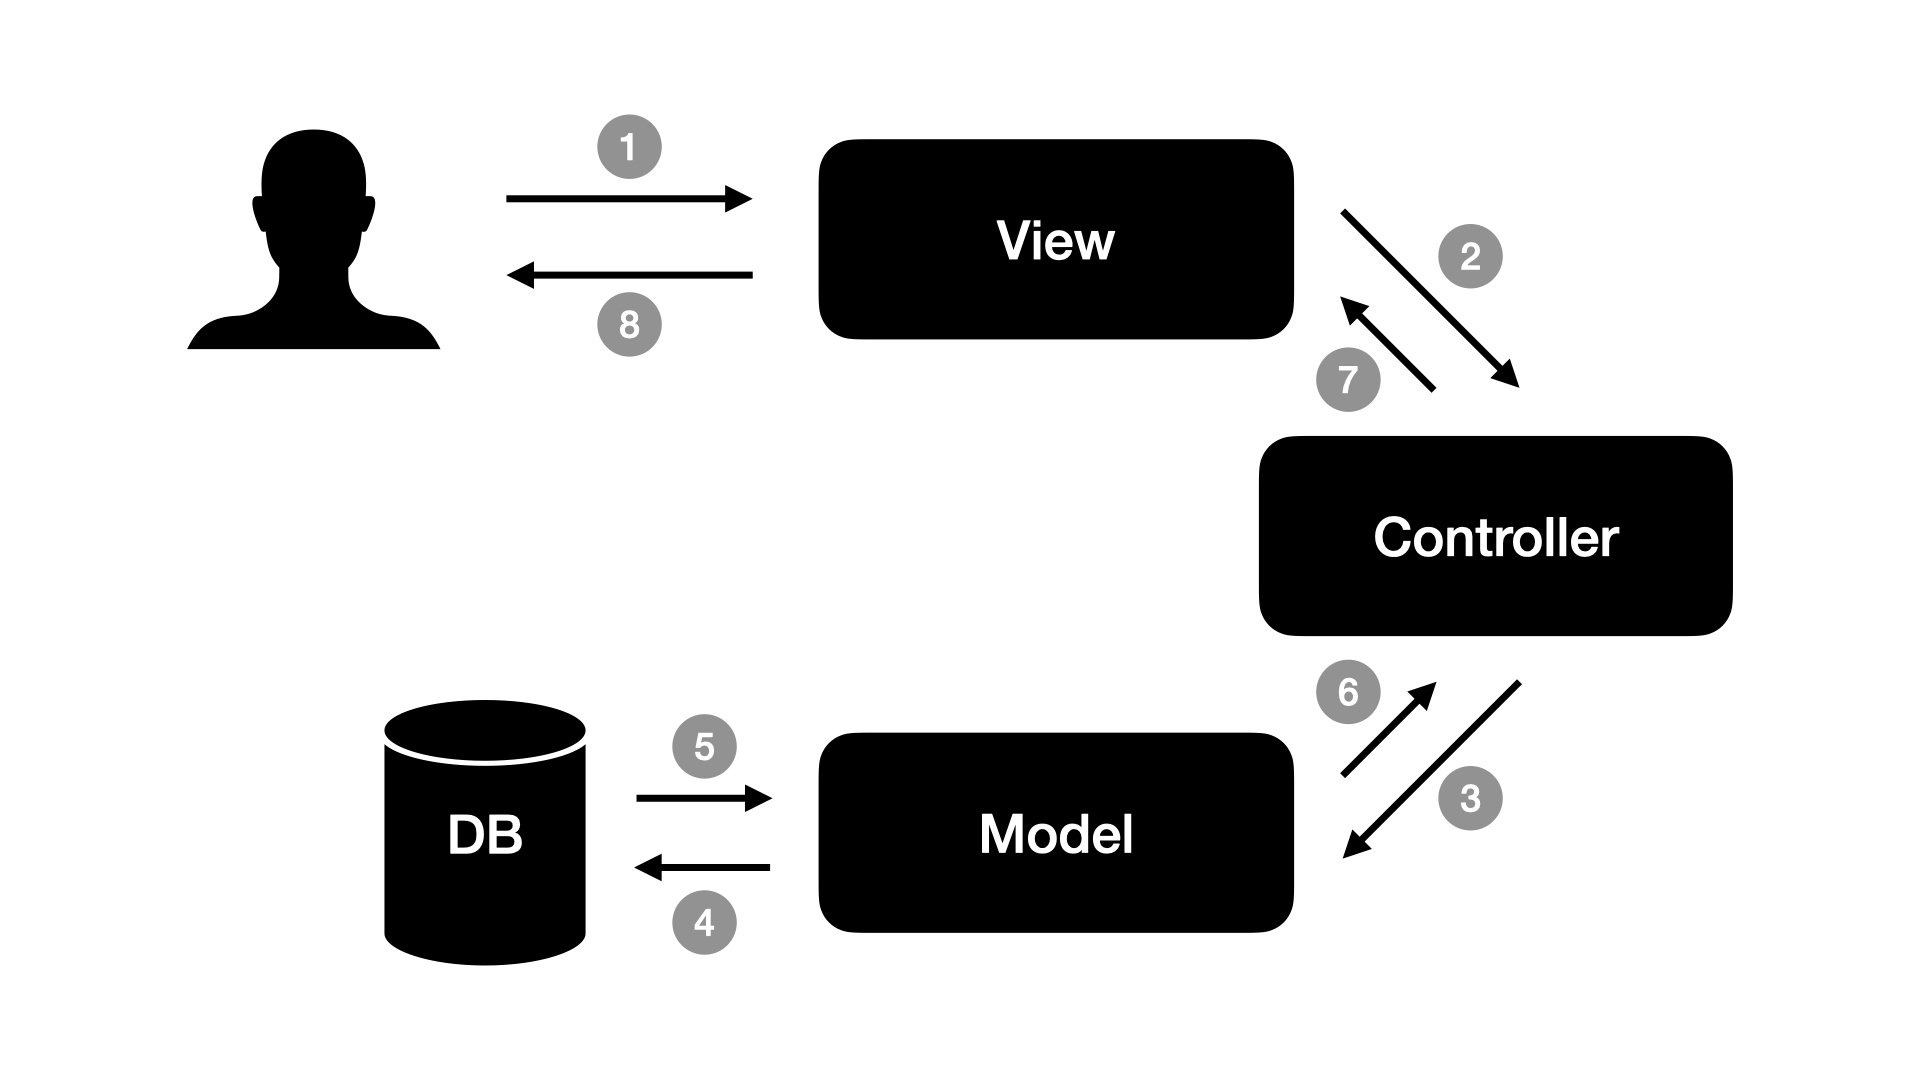
\includegraphics[width=.6\textwidth]{Assets/Interaktionsorientiert.001}
	\caption[Kommunikation zwischen Controller und Model]{Kommunikation zwischen Controller und Model, \\ (1) Der Benutzer sieht die graphische Darstellung und führt eine Aktion aus (2). Der Controller verarbeitet die Aktion und ruft über das Model Daten ab (3). Das Model greift auf die Datenbank zu und lädt die entsprechenden Informationen (4 und 5). Anschließend gibt das Model die Inhalte an den Controller zurück (6). Dieser gibt die Daten an die View weiter (7), welche abschließend die neuen Inhalte dem Benutzer anzeigt (8).}
	\label{fig:mvc-cm-kommunikation}
 \end{figure}
 
 \begin{figure}
 	\centering
    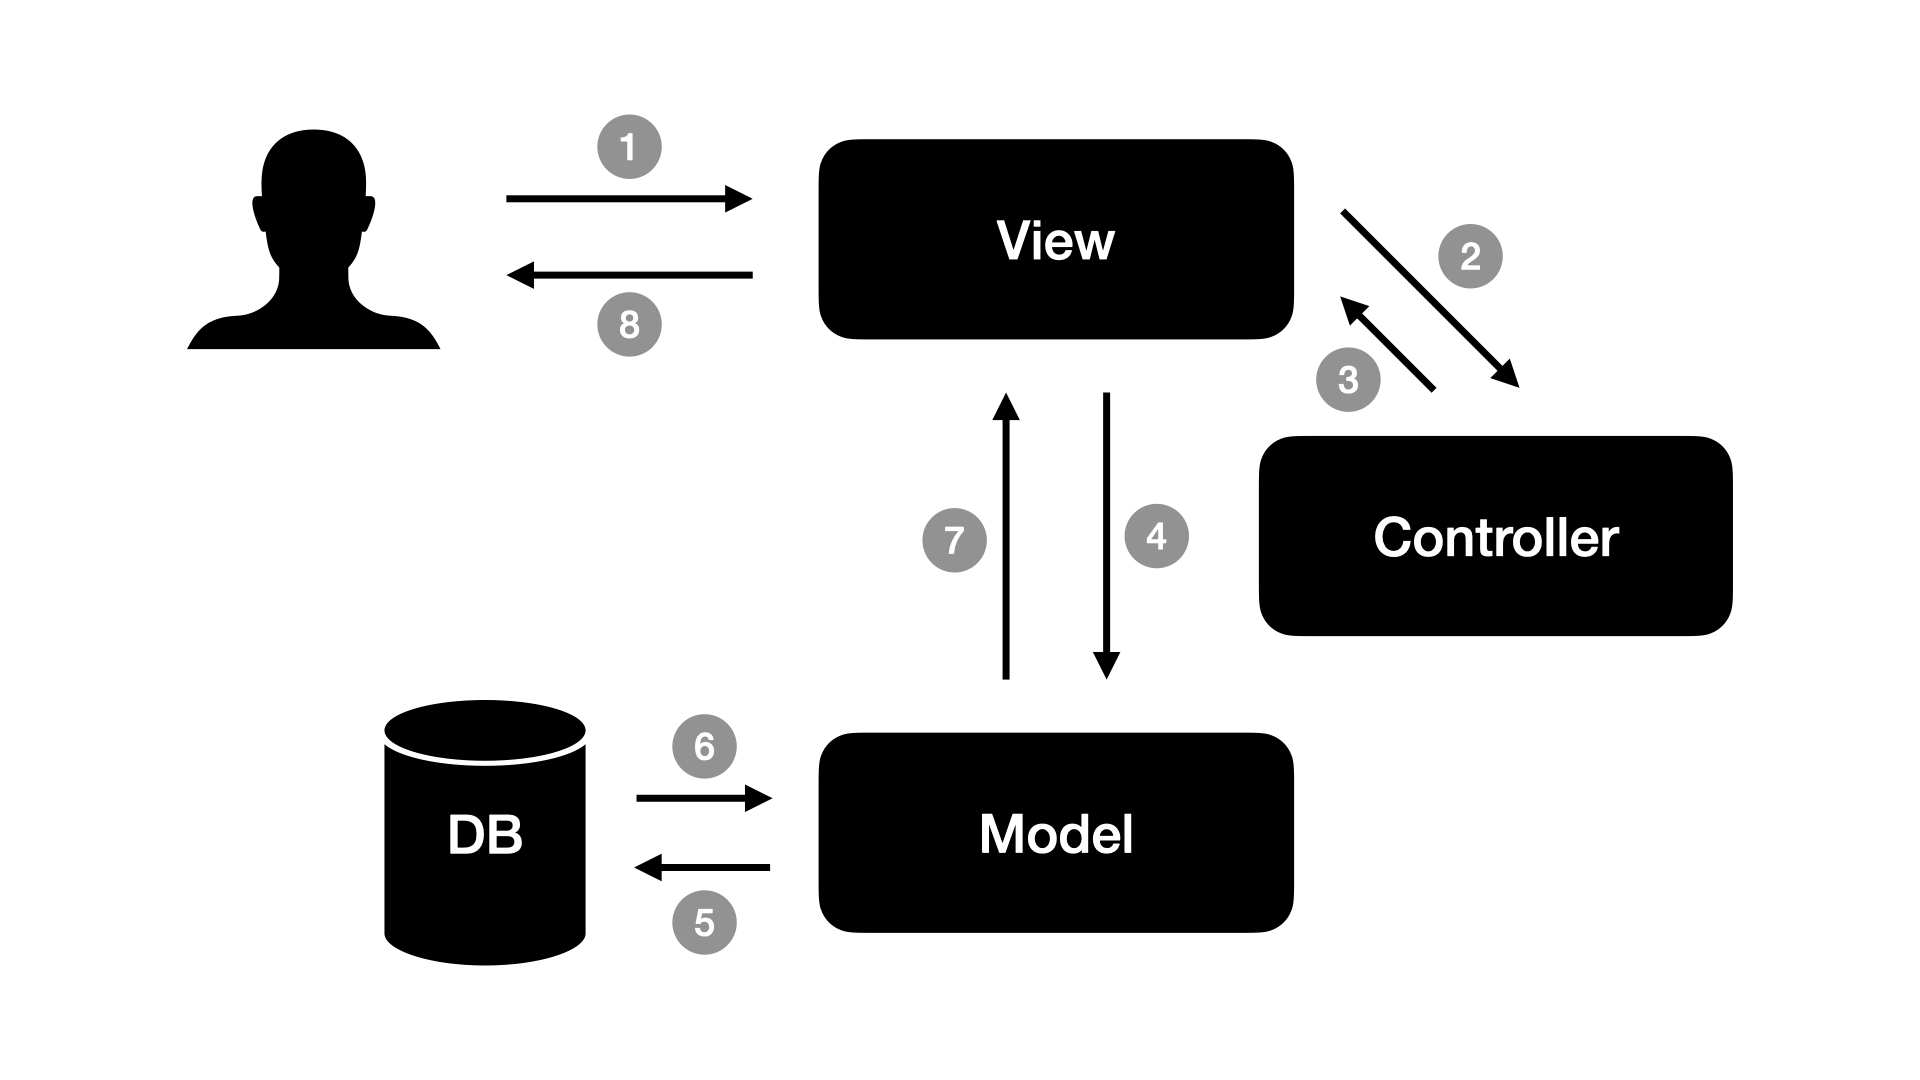
\includegraphics[width=.6\textwidth]{Assets/Interaktionsorientiert.002}
	\caption[Kommunikation zwischen View und Model]{Kommunikation zwischen View und Model, \\ (1) Der Benutzer sieht die graphische Darstellung und führt eine Aktion aus (2). Der Controller verarbeitet die Aktion und rendert umgehend die graphische Darstellung (3). Die View lädt über das Model die Daten (4). Das Model greift auf die Datenbank zu und lädt die angeforderten Informationen (5 und 6). Anschließend gibt das Model die Inhalte an die View zurück (7). Diese zeigt dem Benutzer abschließend die neuen Inhalte an (8).}
    \label{fig:mvc-vm-kommunikation}
 \end{figure}

\subsubsection{REST-Architektur}
\label{sec:rest}

Neben den bislang genannten Architekturstilen, gibt es eine Vielzahl von weiteren Strukturierungen, die sich erst in den letzten 20 Jahre entwickelt haben. Einer dieser Architekturstile ist die REST-Architektur, welche vom Miterfinder des HTTP-Standards, Roy Fielding, definiert wurde \parencite[][S. 128]{starke_effektive_2015}. Er beschrieb diesen Stil in seiner Dissertation an der Universität von Kalifornien im Jahr 2000 und charakterisiert ihn als Architekturstil für das Web.

Dabei steht REST für \textit{Representational State Transfer}, welches einen Architekturstil für verteilte Systeme beschreibt und auf der Client-Server-Architektur aufbaut \parencite[][S. 76]{fielding_architectural_2000}. Client-Server-Architektur beschreibt eine Ausprägung eines verteilten Systems, bei dem die Anwendung in Server und Clients geteilt werden \parencite[][S. 117]{starke_effektive_2015}.\footnote{Dabei beziehen sich die Begriffe \textit{\enquote{Server}} und \textit{\enquote{Client}} auf Software Komponenten und auf den physischen Server und das Endgerät des Nutzers (Client). Des Weiteren grenzt sich der Architekturstil von der Mainframe Architektur ab, bei der über Terminals Anweisungen an einen Großrechner gestellt werden.}

Ein Server ist dabei eine Software Komponente im Netzwerk, welche Services anbietet. Ein Service könnte beispielsweise zuständig sein, alle Informationen der hinterlegten Kunden auszugeben. Der Client hingegen konsumiert lediglich diese Informationen und dient dem Benutzer als Bedienungsoberfläche. Dies bedeutet, dass der Server nur passiv auf Anfragen vom Client wartet, während der Client selbst keine Informationen verarbeitet, sondern ausschließlich anzeigt. Gleichwohl handelt es sich um ein Programm, welches auf dem Endgerät des Benutzers (Computer, Mobiltelefon) ausgeführt wird.

Die REST-Architektur verwendet diese Aufteilung, um eine feste Trennung der Zuständigkeit zu integrieren \parencite[vgl.][S. 78]{fielding_architectural_2000}.

Die zweite Bedingung, die Fielding an den Architekturstil stellt, ist dass die Kommunikation zustandslos, zu Englisch \textit{stateless}, abläuft \parencite[][S. 78]{fielding_architectural_2000}. Dies bedeutet, dass die Nachrichten, die zwischen Server und Client ausgetauscht werden, alle nötigen Informationen beinhalten \parencite[][S. 128]{starke_effektive_2015}. Somit gibt der Server auf Anfrage des Clients stets die gleiche Antwort zurück, egal ob dieser zum Ersten, oder zum wiederholten Mal angefragt wurde. Des Weiteren hängt die Antwort nicht vom Client ab.
Diese Entkopplung zwischen den Komponenten ermöglicht, dass die Aufgabe des Servers, sowie des Clients durch mehrere Computer verrichtet werden kann und  das System skalierbar ist \parencite[][S. 79]{fielding_architectural_2000}.

Der Hauptunterschied zwischen der REST-Architektur und anderen Stilen, liegt in der genauen Bestimmung der zu verwendenden Kommunikationsschnittstellen. So bestimmt die REST-Architektur sehr explizit, welche Form zur Kommunikation verwendet werden darf. So werden Methoden vom Server über HTTP-Standards aufgerufen. Konkret bedeutet dies, dass die einzelnen Dienste des Servers sich nach den HTTP-Methoden (GET, PUT, POST und DELETE) richten und es ein klares Mapping zwischen ihnen gibt. \parencite[vgl.][S. 128]{starke_effektive_2015}. Somit baut die REST-Architektur auf einem Kommunikationsstandard auf, der sich im Internet etabliert hat.

Auf Grundlage der standardisierten Kommunikation können zwischen Server und Client intelligente Zwischenstationen geschaltet werden, die dafür zuständig sind, häufig vorkommende Anfragen abzuspeichern \parencites[vgl.][S. 79 f.]{fielding_architectural_2000}[][S. 128]{starke_effektive_2015}.

Die Antwort des Servers erfolgt durch Repräsentationen der Daten, wovon es für jede Ressource\footnotemark mehrere Formate gibt. So kann eine Schnittstelle abhängig vom Aufruf sowohl JSON, als auch XML oder HTML zurückgeben \parencite[vgl.][S. 128]{starke_effektive_2015}.
\footnotetext{Als Ressource werden die Informationen bezeichnet, die durch den Aufruf einer URL zurück gegeben werden. Ein Beispiel wäre der HTTP-Aufruf \textit{GET: https://api.plurapolit.de/api/users}, der alle Informationen der User zurück gibt.}

Verwendet wird die REST-Architektur ausschließlich für Anwendungen im Internet, da es auf die Anwendung des Hypertext Transfer Protokoll\footnote{Weitere Informationen zum Hypertext Transfer Protokoll kann unter folgender Literatur gefunden werden \parencite{leach_hypertext_2020}.} (HTTP) angewiesen ist. Dabei findet der Architekturstil sowohl Anwendung für ganze Systeme, als auch für komplexe Anwendungen mit einer Vielzahl einzelner Services.

\subsubsection{Monolithische Architektur}
\label{sec:monolith}

Der Begriff \textit{\enquote{Monolith}} leitet sich vom altgriechischen \textit{\enquote{monólithos}} ab und bedeutet \textit{\enquote{aus einem Stein}} \parencites[vgl.][]{duden_nodate}[vgl.][]{dwds_nodate}. In der Gesteinskunde wird damit ein natürlich entstandener Gesteinsblock bezeichnet, der komplett aus einer Gesteinsart besteht \parencite[vgl.][]{dwds_nodate}.

Nach Rod Stephens liegt eine monolithische Softwarearchitektur vor, wenn jegliche Funktionalität des Systems miteinander verbunden ist. Dabei spricht er über die Verbindung von Dateneingabe, Datenausgabe, Datenverarbeitung, sowie Fehlerhandhabung und Benutzeroberflächen \parencite[vgl.][S. 94]{stephens_beginning_2015}.

Anders sieht es Sam Newman. Nach ihm liegt ein monolithisches System schon dann vor, wenn die gesamte Funktionalität eines Systems gemeinsam über einen Deployment-Prozess\footnotemark bereitgestellt wird \parencite[vgl.][Kap. 2.2]{newman_monolith_2019}. Folglich muss nicht zwingend jegliche Logik miteinander verbunden sein. Er unterteilt monolithische Systeme in drei Kategorien: Einzelprozess-Monolithe, modulare Monolithe und verteilte Monolithe \parencite[vgl.][Kap. 2.2]{newman_monolith_2019}.
\footnotetext{Deployment-Prozess, oder auch Bereitstellungsprozess, bezeichnet den Prozess ein Software-System Benutzern zur Verfügung zustellen \parencite[vgl.][]{softwareverteilung_2020}.}

Der Einzelprozess-Monolith ist die gängigste Form und deckt sich mit der Definition von Rod Stephens. Es handelt sich dabei, um ein System bei dem das gesamte System einen Prozess abbildet. Dies bedeutet, dass jegliche Funktionalität aufeinander aufbauend ist und nur eine Datenspeicherung für die gesamte Anwendung verwendet wird \parencite[vgl.][Kap. 2.2.1]{newman_monolith_2019}.

Anders ist dies bei dem modularen Monolithen. Er zeichnet sich darin aus, dass die Funktionalität in einzelne Module geteilt wird, die eine separate Datenspeicherung besitzen können \parencite[vgl.][Kap. 2.2.2]{newman_monolith_2019}. Im Gegensatz zu verteilten Systemen sind die einzelnen Module jedoch nicht auf separaten Computern verteilt, sondern über einen Rechner online gestellt. Des Weiteren sind die einzelnen Module nur leicht entkoppelt, sodass es zwischen ihnen Abhängigkeiten geben kann.

Dies ist bei verteilten Monolith anders, da die einzelnen Module komplett entkoppelt sind und Nachrichten ausschließlich über definierte Schnittstellen ausgetauscht werden \parencite[vgl.][S. 116]{starke_effektive_2015}. Ein verteilter Monolith erfüllt somit jegliche Anforderungen an ein verteiltes System mit der Ausnahme, dass alle Komponenten durch nur einen Prozess online gestellt werden.

Weder Stephens noch Newman geben Vorgaben hinsichtlich der Gliederung innerhalb eines monolithischen Systems. Demnach kann ein MVC-Ansatz als monolithisches System gelten, solange es einheitlich bereitgestellt wird.

Im Rahmen dieser Arbeit wird beim Begriff Monolith stets von einem Einzelprozess-Monolithen ausgegangen, außer es wird explizit von einem modularen, oder verteilten Monolithen geschrieben.

Vergleicht man das monolithische System mit einem verteilten System, gibt es Vor- und Nachteile \parencite[vgl.][Kap. 2.2.4 und Kap. 2.2.5]{newman_monolith_2019}. So ist das Bereitstellen eines Monoliths einfacher, da es einen Bereitstellungsprozess für die gesamte Anwendung gibt. Wiederum führt dies dazu, dass der Prozess deutlich länger dauert. Diese Tatsache ist besonders dann gravierend, wenn vermehrt kleine Änderungen vorgenommen werden. Andererseits vereinfacht eine Anwendung, die als ein Prozess zu sehen ist, die Fehlersuche und ermöglicht es Funktionen mehrfach zu verwenden. Das verursacht jedoch, dass schnell Abhängigkeiten entstehen können und Änderungen ungewollte Fehler verursachen. Dadurch wird die Umsetzung von neuen Funktionen mit wachsender Codebase verlangsamt und der Einstieg von neuen Teammitgliedern erschwert.

Da alle Entwickler eines Unternehmens auf einer Codebase arbeiten, kommt es schnell zu Unterschieden im Programmcode. So führt ein Monolith dazu, dass bei einer großen Anzahl von Entwicklern viele Absprachen notwendig sind \parencite[vgl.][Kap. 2.2.4]{newman_monolith_2019}.

Anders ist es bei systemübergreifenden Tests: Diese werden durch ein monolithisches System begünstigt und können im Vergleich zu einem verteilten System einfacher umgesetzt werden  \parencite[vgl.][Kap. 2.2.5]{newman_monolith_2019}.

\subsubsection{Einordnung des aktuellen Systems von PluraPolit}
\label{sec:einordnung}

Wie bereits in der Einleitung beschrieben, bietet PluraPolit eine Plattform an, die Jung- und Erstwähler bei der politischen Bildung unterstützt.

Es wurde ein Software-System entwickelt, welches auf der einen Seite PluraPolit die Möglichkeit gibt Content zu verwalten und auf der anderen Seite dem Endkunden die Inhalte graphisch aufbereitet. Hierfür wurde, neben der Plattform für die Nutzer, ein Content Management System (CMS) umgesetzt. Programmiert wurde dieses im  Webframework Ruby on Rails.\footnote{
Ruby on Rails, kurz auch als Rails bezeichnet, ist ein quellenoffenes Webframework, welches für die Programmiersprache Ruby entwickelt wurde \parencites[vgl.][S.4]{hartl_ruby_2016}{ruby_org}[vgl.][S. 24]{sieben_wochen}. Es ist komplett Open Source und wird von einer aktiven Community entwickelt. Es gibt eine Vielzahl von kostenfreien Paketen, sogenannte Gems, die nach Belieben zu einem Projekt hinzugefügt werden können. Im Vergleich zu anderen Frameworks zeichnet sich Rails besonders durch seine Implementierung der REST-Architektur aus \parencite[vgl.][S. 5]{hartl_ruby_2016}. Diese Implementierung führt jedoch dazu, dass eine Vielzahl von Bedingungen an die Entwicklung und Implementierung von Rails-Anwendungen gestellt werden. Getreu dem Motto \textit{\enquote{Konvention vor Konfiguration}} nutzt Rails die Bestimmungen als Vorteil und integriert ein System, in das externe Pakete ohne Konfigurationsaufwand hinzugefügt werden können \parencite{ruby_doctrine}.
} Strukturiert werden Rails-Anwendungen nach dem MVC-Ansatz \parencites[vgl.][S. 66 ff.]{hartl_ruby_2016}.

\begin{figure}
	\centering
	\begin{subfigure}[a]{0.4\linewidth}
		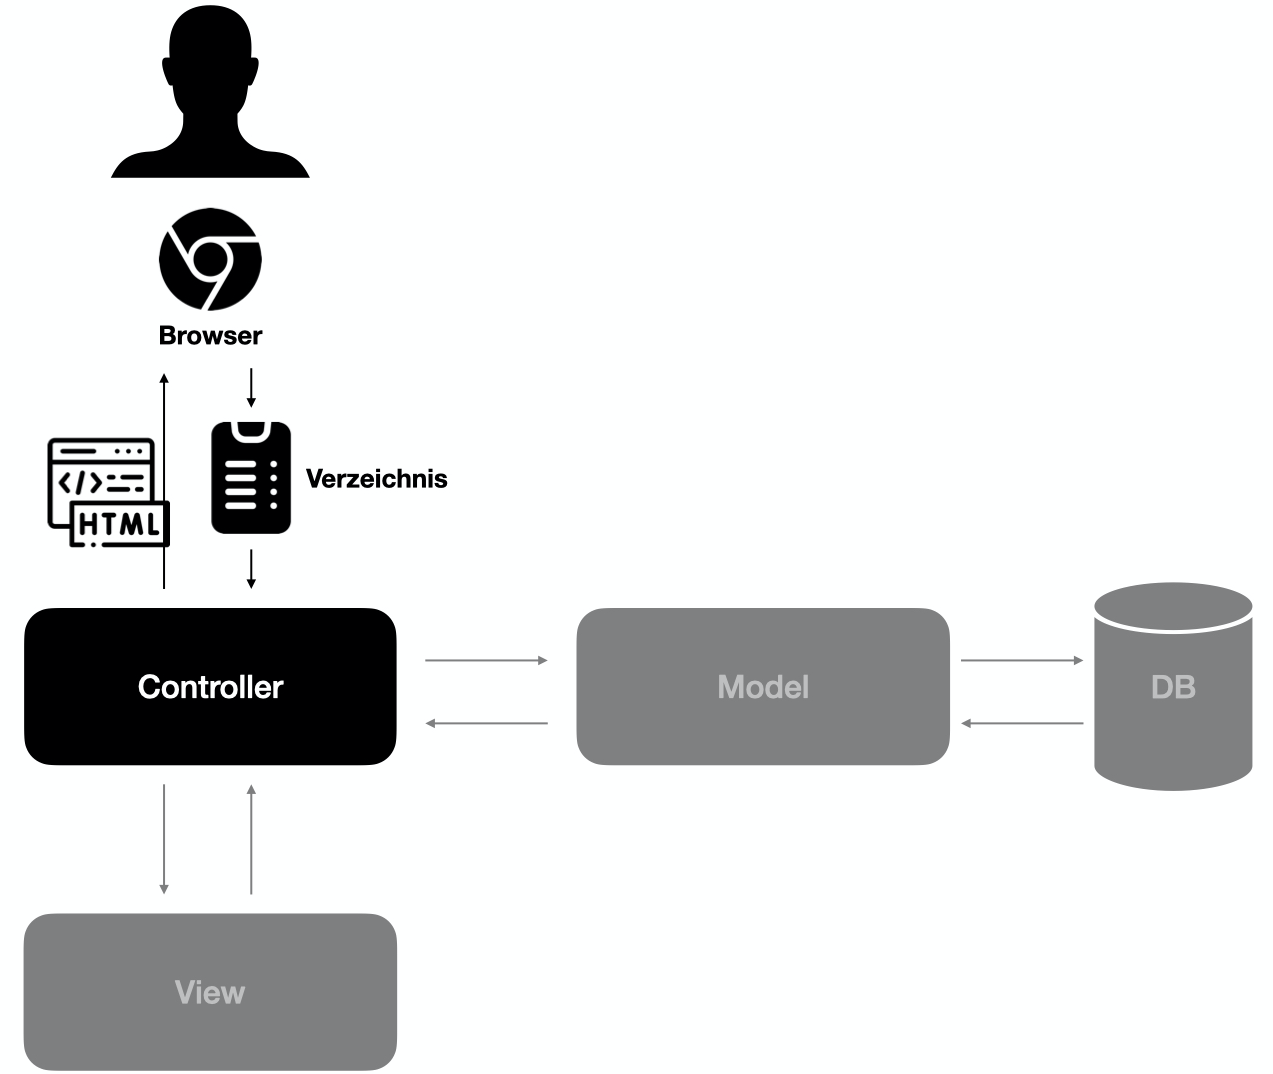
\includegraphics[width=\linewidth]{Assets/PluraPolit-Softwaresystem.001}
		\caption{Aufruf der Webseite}
		\label{fig:plurapolit-call-webpage}
	\end{subfigure}
	\begin{subfigure}[a]{0.4\linewidth}
		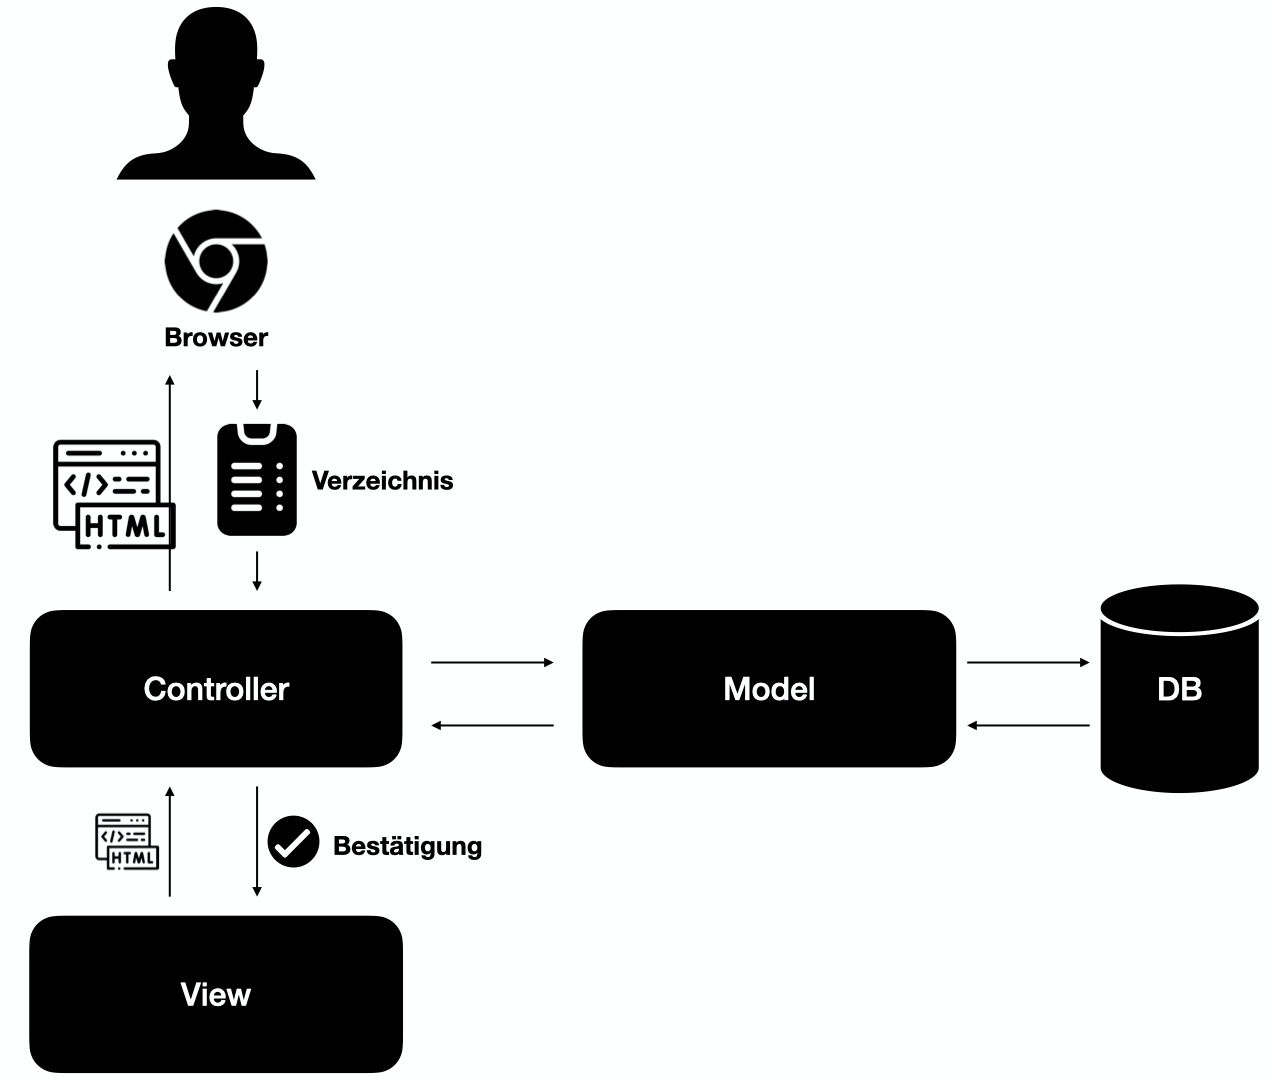
\includegraphics[width=\linewidth]{Assets/PluraPolit-Softwaresystem.002}
		\caption{Abspeichern der Tondatei}	
		\label{fig:plurapolit-save-sounddatei}
	\end{subfigure}
	\begin{subfigure}[b]{0.4\linewidth}
		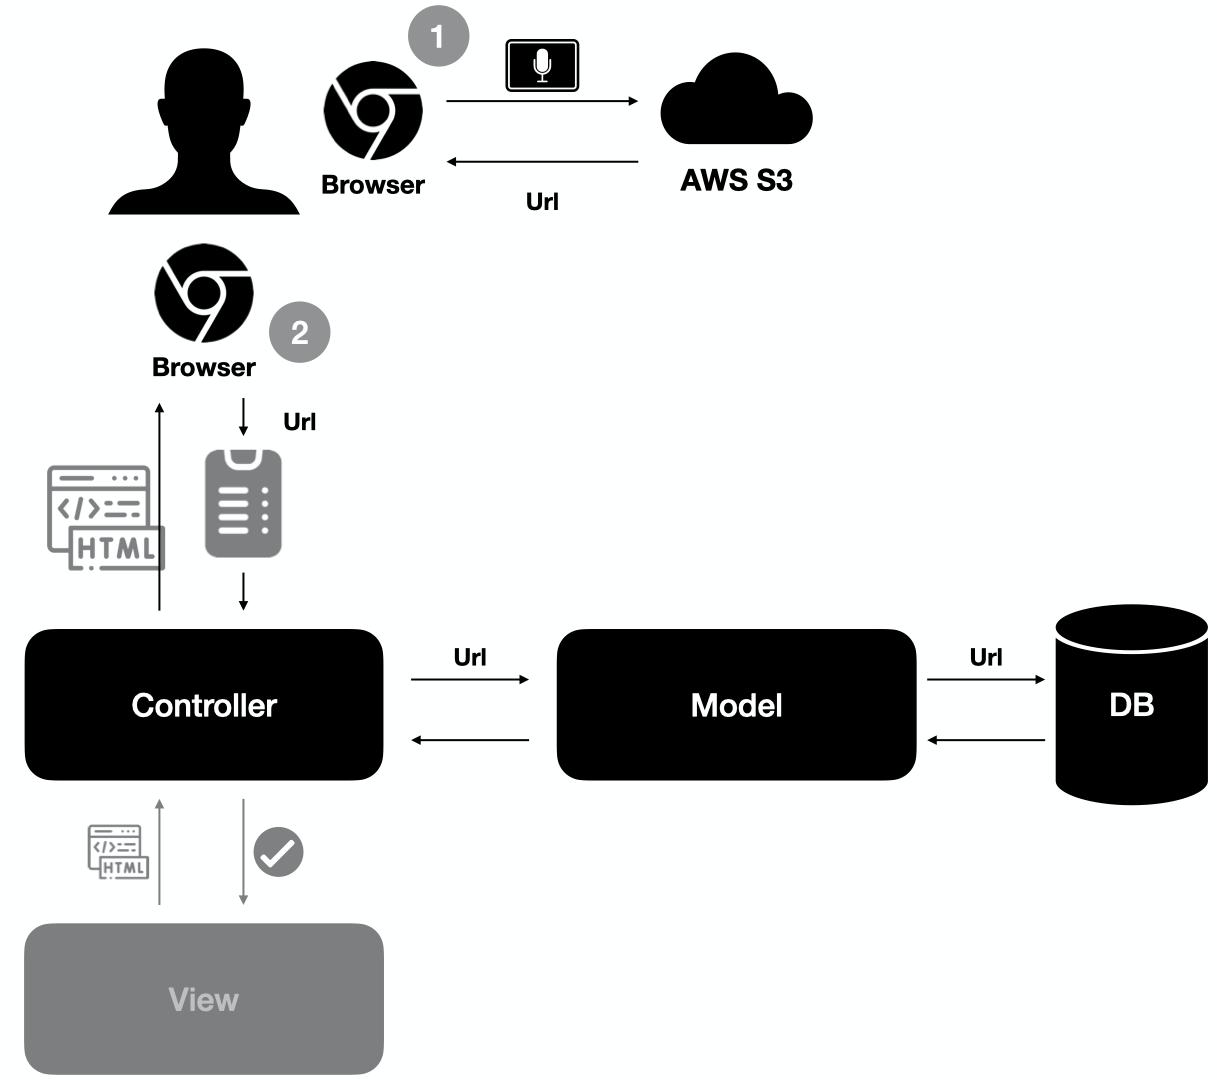
\includegraphics[width=\linewidth]{Assets/PluraPolit-Softwaresystem.003}
		\caption{Speichern zu S3}
		\label{fig:plurapolit-save-to-s3}
	\end{subfigure}
	\caption{Speichern einer Tonaufnahme}
	\label{fig:coffee}
\end{figure}

Um eine neue Tonaufnahme einzupflegen, wird die entsprechende Webseite im Browser aufgerufen. Dabei sendet der Browser über die URL eine Anfrage an den Server, der anhand eines Verzeichnises den verantwortlichen Controller bestimmt und die Anfrage an diesen weiterleitet.  Der Controller verarbeitet die Anfrage und schickt eine HTML-Seite zurück (siehe \cref{fig:plurapolit-call-webpage}).

Über diese Webseite kann die Aufnahme hochgeladen und abgespeichert werden. 
Dies geschieht, indem per Klick im CMS eine HTTP-Anfrage an den Controller geschickt wird. Der Controller speichert den Eintrag und bestätigt das erfolgreiche Abspeichern im View. Das Speichern geschieht dabei über das Model (siehe \cref{fig:plurapolit-save-sounddatei}).

Dabei wird die Tondatei selbst nicht in der Datenbank gespeichert, sondern lediglich ein Verweis darauf. 
Die Datei wird vorher zum Speicherservice von Amazon Web Services (S3) geschickt, welcher die Tonaufnahme über eine URL zur Verfügung stellt. Nur die URL wird in die Datenbank hinterlegt (siehe \cref{fig:plurapolit-save-to-s3}).

\begin{figure}
	\centering
	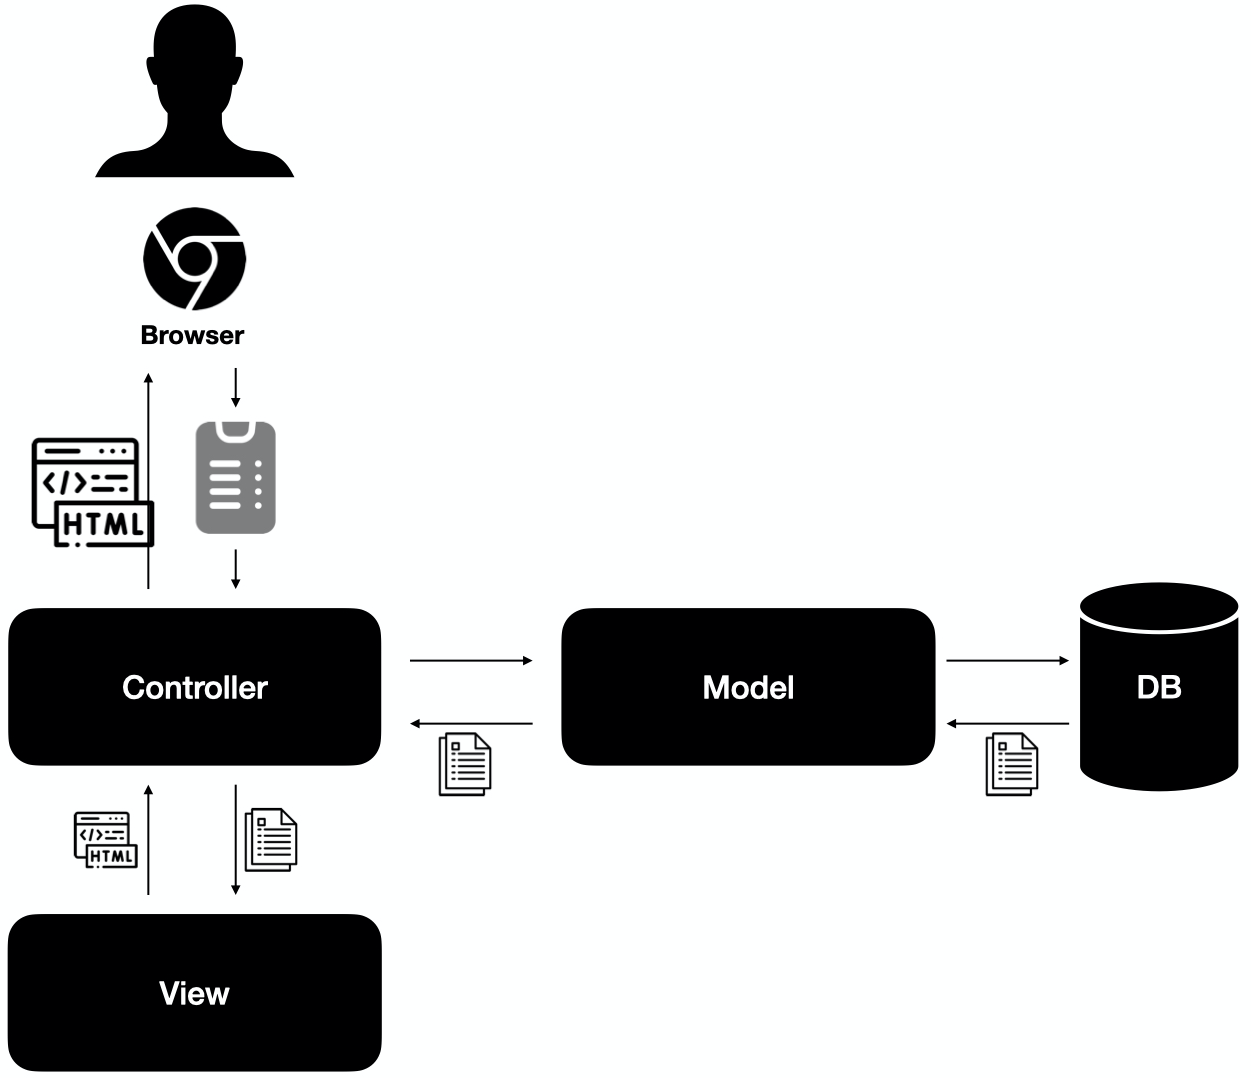
\includegraphics[width=0.5\linewidth]{Assets/PluraPolit-Softwaresystem.004}
	\caption{Inhalte bearbeiten}
	\label{fig:plurapolit-edit}
\end{figure}

Neben dem Abspeichern der Tonaufnahmen kann das CMS auch zum Bearbeiten und Anpassen von bestehenden Datensätzen genutzt werden. Hierfür wird die jeweilige Webseite aufgerufen, welches dazu führt, dass der Controller die angeforderten Daten aus der Datenbank lädt und die entsprechende graphische Darstellung an den Browser zurück gibt. Dabei greift der Controller nicht direkt auf die Datenbank zu, sondern lädt die Inhalte über das Model.
Auch übergibt der Controller lediglich die geladenen Inhalte an die View, welche  die Daten über Embedded Ruby in das HTML Template integriert und die fertige Webseite zurück gibt (siehe \cref{fig:plurapolit-edit}).

\begin{figure}
	\centering
	\begin{subfigure}[c]{0.3\linewidth}
		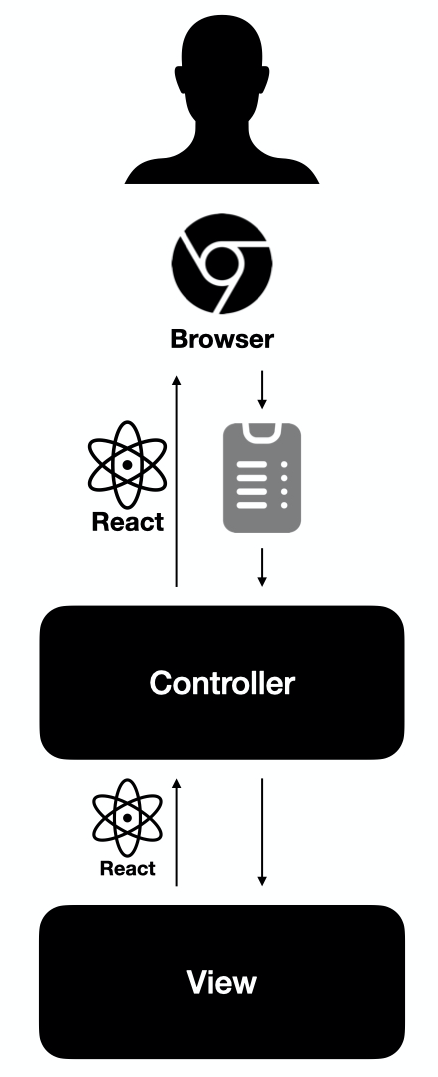
\includegraphics[,height=7cm]{Assets/PluraPolit-Softwaresystem.005}
		\caption{React-App aufrufen}
		\label{fig:plurapolit-load-react}
	\end{subfigure}
	\begin{subfigure}[c]{0.6\linewidth}
		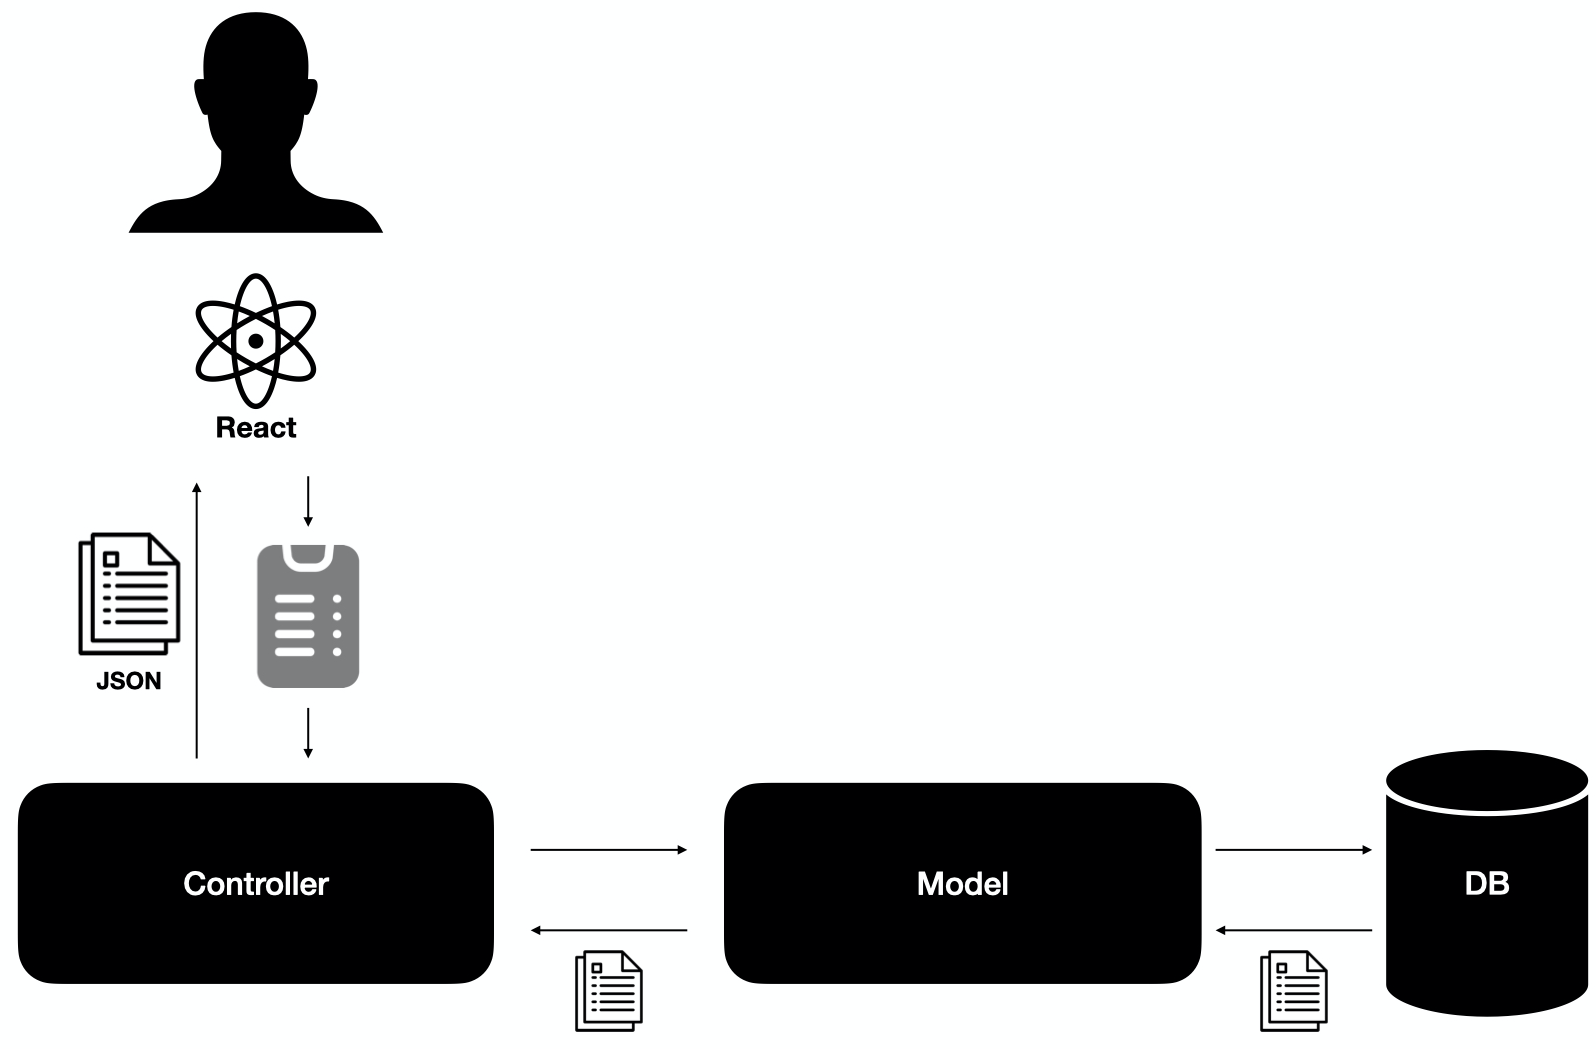
\includegraphics[width=\linewidth]{Assets/PluraPolit-Softwaresystem.006}
		\caption{React-App lädt Inhalte}
		\label{fig:plurapolit-react-data}
	\end{subfigure}
	\caption{Endkunde lädt die Plattform}
\end{figure}

Bei der Plattform für die Endkunden handelt es sich, um die selbe Anwendung wie beim CMS, mit dem Unterschied, dass die graphischen Darstellung durch eine React-Anwendung\footnotemark übernommen wird. So wird beim Aufruf der Plattform eine Anfrage an den Controller geschickt, der anschließend die kompilierte React-Anwendung zurück gibt (siehe \cref{fig:plurapolit-load-react}).

\footnotetext{Eine React-Anwendung oder auch React-App ist eine Webanwendung, die in React.js programmiert ist \parencite{react-anwendung}.}

Diese lädt eigenständig jegliche Informationen über HTTP-Anfragen und kümmert sich um interne Seitenaufrufe. Die Anfragen werden dabei asynchron an die Rails-Anwendung geschickt und vom Controller beantwortet. Über die Kommunikation von Controller und Model erhält die React-Anwendung den Content aus der Datenbank, der vorher eingepflegt wurde (siehe \cref{fig:plurapolit-react-data}).

Es gibt also eine Aufteilung bezüglich der graphischen Darstellung in Content Management System und Plattform. Die Datenspeicherung und Verwaltung sind jedoch gleich. Die gesamte Codebase wird in einem Bereitstellungsprozess dem Hosting Service zur Verfügung gestellt. Damit handelt es sich bei dem System von PluraPolit um ein Monolith, welches teilweise modular ist, die REST-Standards erfüllt und nach dem MVC-Ansatz strukturiert ist. Des Weiteren nutz das System vereinzelt externe Services von AWS, um Tondateien zu speichern.
